\section{ミニアプリとの対応}
\label{sec:ミニアプリ}

\subsection{はじめに}

計算機ハードウェア・ソフトウェアの性能や機能を評価するためにベンチマークソフトウェアが用いられているが、それらは典型的にはアプリケーションから限られた一部を切り出したプログラムであったり、人工的に作成されたプログラムである。カーネルベンチマークと呼ばれるこれらの評価用プログラムは、通常のアプリケーションと比較してそのサイズは大幅に小さいものであり、システムの評価に用いやすい利点がある。一方で、カーネルベンチマークは実際のアプリケーションのごく一部のみを反映したものであり、実際のアプリケーション全体を評価できているとは限らない。しかしながら、特に開発途中のシステムの評価に巨大な実アプリケーションを用いることは技術的に困難であり、カーネルベンチマークのような簡易なプログラムが必要である。

より実際のアプリケーションに即しつつ、プログラムサイズを比較的小さなものとし評価に利用し易くすることを目的としたベンチマークとして、ミニアプリベンチマークが提唱されている。ミニアプリは実アプリケーションから評価に必要な箇所を残し、それ以外の非本質的なコードを可能な限り削除することでプログラム全体の見通しを改善する。また、コンパイル方法や実行方法などの文書化、入力データの整備などがあわせて必要である。実アプリケーションには限定的なライセンスにより配布が制限されているものも多いが、そのような制約は限定された範囲内における利用で問題とならないかもしれないが、第三者によるベンチマークとしての利用の場合は利用に関する制約は大きな障害となりうる。そのためミニアプリが非公開アプリケーションから作成された場合であってもミニアプリについてはオープンソースとすることが一般的である。

上記のような背景のもとに作成されたミニアプリは特にアプリケーションと計算機システムのコデザインに有効なツールとして用いられている。特に代表的なものとしては米国のコデザインセンターを中心に開発されたMantevoやLuleshなどがあげられる。国内では理化学研究所が中心となって整備したFiberがあげられる。以下ではそれらについて概要を紹介し、本ロードマップのアプリケーションとの比較を示す。

\subsection{Fiberミニアプリ}
Fiberミニアプリ集(Fiber Miniapp Suite)~\cite{Fiber}は、理化学研究所および東京工業大学にて実施した「将来のHPCIシステムのあり方の調査研究「アプリケーション分野」」~\cite{ApliFS}(以下、アプリFSと呼ぶ)において整備開発したミニアプリ群をまとめたものである。
%アプリFSでは、2018〜2020年頃の社会的・科学的課題を担うアプリケーションの調査を国内の数多くの計算科学者の協力の下、2012年度から2013年度にかけて実施され、その調査結果は「計算科学ロードマップ(2014年3月版)」としてまとめられた~\cite{Roadmap_2014}。
アプリFS参加協力者から提供されたアプリケーションプログラムをベースに、
完成後の一般公開を前提に、オリジナルアプリケーション開発者の協力のもとでミニアプリの整備開発が行われた。
2017年3月現在、
著作権や性能面などでの問題が解決できなかったものを除いた、
8つのミニアプリをWeb上で公開している。

Fiberでは、前節で示した一般的なミニアプリの共通点の他に、
以下のような特徴を持ったミニアプリ集を目標とした。

\begin{itemize}
\item 簡単にインストール、簡単にに実行
\item 正しくインストールされ、正しく実行されていることが検証可能なテスト
\item システムの性能評価に使える入力データセット
\item 将来(2018〜2020年頃)の想定計算対象規模とそこでの目標性能に関する記述を含めたドキュメントの整備
\end{itemize}

また、その開発経緯により、ミニアプリ化されたアプリケーションは全て国内で開発されたものであり、
事実上国内固有のアーキテクチャである京コンピュータ上でのインストール・実行が保証されている。

以下では、Fiberとして公開中の各ミニアプリに対して、
計算対象と計算手法、使用言語と並列化ライブラリ、どのようにミニアプリ化したか、
ソースコードサイズ、付随する入力データ、などを中心に簡単に紹介する。

\rmproject{CCS QCD}
ミニアプリCCS QCD~\cite{CCS-QCD_boku2012,CCS-QCD_terai2013}は、
高エネルギー物理学で用いられる格子量子色力学(格子QCD)計算における、
最も計算コストがかかるクォーク伝搬関数の計算部部分を抜き出したものである。
CCS QCDでは、Wilson型の作用を用いたクォーク伝搬関数の4次元格子上での大規模疎行列連立1次方程式を、
red/black orderingにより前処理をした係数行列に対して、BiCGStab法により解いている。
プログラムはFortran90で記述され,並列化は,空間3次元に対するMPI領域分割とOpenMPスレッド並列を行っている。
コメント行を除いたソースコードサイズは約1千行である。
パッケージには、強スケーリングおよび弱スケーリングでの性能計測に対応可能な6つの入力データセットが含まれている。

\rmproject{FFVC Mini}
ミニアプリFFVC Miniは,直交等間隔格子上の有限体積法による熱流体解析プログラムFFV-C~\cite{FFVC_ono2014}をベースとしている。
プログラム全体の制御はC++で記述されているが、ホットスポット部分はFortran90により書かれている。
空間3次元に対するMPI領域分割とOpenMPにより並列されている。
ミニアプリ化にともない、計算対象を非圧縮流体に対する3次元キャビティ流れに限定した。
コメント行を除いたソースコードサイズは約9000行である。
ミニアプリ内で、強スケーリングおよび弱スケーリングでの性能計測に対応可能なグリッドデータを自動生成する。

\rmproject{NICAM-DC Mini}
ミニアプリNICAM-DC Miniは、
全地球規模での気象現象をシミュレーションする大気大循環モデルのアプリケーションNICAM~\cite{NICAM_satoh2008}のサブセットNICAM-DC~\cite{NICAM-DC_url}をベースにしている。
NICAM-DCは、NICAMから力学過程(Dinamical Core)のみを抜き出したミニアプリとなっている。
NICAM-DCでは、地球大気の運動を静水圧近似を行わないNavier-Stokes方程式で記述し、
それを球殻上の三次元格子を用いて有限体積法により離散化して解いている。
水平方向の格子は、正二十面体を構成する正三角形要素を再帰的に分割していくことにより得られる全球で一様な三角格子を採用している。
%時間積分は。水平方向はRunge-Kutta法により陽解法で、鉛直方向は陰解法として1次元Helmholtz方程式を離散化した三重対角行列を係数に持つ連立一次方程式を解くことにより進めている。
NICAM-DCは、Fortran90で記述され、MPIによる領域分割並列化がなされている。
コメント行を除いたソースコードサイズはは3万5千行である。
ミニアプリNICAM-DC Miniには、強スケーリングおよび弱スケーリングでの性能計測に対応可能な5つの入力データセットが付随している。

\rmproject{mVMC Mini}
ミニアプリmVMC Miniは、強相関電子系シミュレーションプログラムmVMC~\cite{mVMC_url,mVMC_tahara2008}をベースとしている。
mVMCは,近藤格子などの多体量子系有効模型の基底状態の波動関数を多変数変分モンテカルロ法により求める。
mVMCは、C言語で記述され、MPIおよびOpenMPにより並列化されている。
コメント行を除いたソースコードサイズは約9千行である。
ミニアプリmVMC Miniには、強スケーリングおよび弱スケーリングでの性能計測に対応可能な2つの入力データセットが付随している。

\rmproject{NGS Analyzer Mini}
ミニアプリNGS Analyzer MiniのベースとなったNGS Analyzerは、
次世代シークエンサーの出力データを高速に解析し、
ヒト個人間の遺伝的差異やがんゲノムの突然変異を高い精度で同定するプログラムである~\cite{NGSA_url}。
NGS Analyzer Miniは、NGS Analyzerを大規模I/O性能および整数演算性能を評価するためのミニアプリとして整備したものである。
2つのオープンソースソフトウェアを含む4つのC/C++プログラムと、ワークフローを制御するMPI並列化されたCプログラムとシェルスクリプト群で構成され、オープンソースソフトウェアを除いた総コードサイズは約3千行である。
入力データはサイズが大きいため、付属ドキュメントの記述に従い、別途ダウンロードする必要がある。

\rmproject{MODYLAS Mini}
ミニアプリMODYLAS Miniは、古典分子動力学シミュレーションプログラムMODYLAS~\cite{Modylas_url,Modylas_andoh2013}をベースにしている。
MODYLASでは、クーロン相互作用を、八分木構造を持つ空間セル上での多重極展開計算により計算するFast Multipole Method (FMM)法を採用している。
MODYLASはFortran90で記述され、MPIおよびOpenMPによる並列化がなされている。
ミニアプリ化にともない、計算対象を水分子系のミクロカノニカル計算に限定している。
コメント行を除いたソースコードサイズは8.7千行である。
パッケージには、強スケーリングおよび弱スケーリングでの性能計測に対応可能な3つの入力データセットが付随している。

\rmproject{NTChem Mini}
ミニアプリNTChem Miniは、第一原理計算にもとづく電子状態計算プログラムNTChem~\cite{NTChem_url}のサブパッケージNTChem/RI-MP2~\cite{NTChem_katouda2013}をベースにしている。
NTChem/RI-MP2では、電子相関を2次のM{\o}ller-Plesset摂動(MP2)法に対するresolution-of-identity(RI)近似を用いて計算しており、
演算は密行列に対する行列行列積計算が中心となる。
NTChem/RI-MP2は、Fortran90で記述され、MPIおよびOpenMPにより並列化されている。
コメント行を除いたソースコードサイズは約6.5千行である。
ミニアプリNTChem Miniには小規模分子系のサンプル入力データのみが付属するが、
別途、強スケーリング性能計測に対応可能な入力データがダウンロード可能である。

\rmproject{FFB Mini}
ミニアプリFFB Miniは、有限要素法による熱流体解析プログラムFrontFlow/blue (FFB)~\cite{FFB_minami2012,FFB_kumahata2013}をベースにしている。
ミニアプリ化にあたり、計算対象を六面体要素に対する基本的な非定常流体解析計算に限定した。
FFB MiniはFortran90で記述され、MPIにより3次元領域分割並列化に対応している。
また、京コンピュータおよび富士通FX10上での、自動並列によるスレッド並列計算に対応している。
コメント行を除いたソースコードサイズは約8千行である。
ミニアプリ内で、強スケーリングおよび弱スケーリングでの性能計測に対応可能なグリッドデータを自動生成する。

\subsection{その他のミニアプリ関連プロジェクト}
\label{sec:その他のミニアプリ}

海外においてもFIBERと同様にミニアプリを整備して性能評価用の共通情報資源
として活用しようとする動向がある。

\subsubsection{米国のミニアプリ関連 - CORALプロジェクト}
米国においては米国エネルギー省の管轄下にある
Argonne国立研究所、Lawrence Livermore国立研究所、Oak Ridge国立研究所の
3研究所のHPC調達共通化にともない、性能評価用に用いられるCORALベンチマーク
が公開されている\cite{CORAL-benchmarks,CORAL-slides}。
CORALベンチマークの内 LSMS, CAM-SE, QMCPACK, NAMD を除き、アプリは基本的に
ミニアプリである。

\begin{table}[H]
%	\begin{table}[htb]
\caption{CORAL benchmarks (tier1およびtier2 アプリのみ掲載)}
\label{tab:CORAL-apps-names}
{
%\tiny
%\scriptsize
%\footnotesize
%\small
%\normalsize
\begin{tabular}{p{75mm}|p{75mm}} \hline
%	\begin{tabular}{l|l} \hline
アプリ名 &	CORALによるジャンル分け \\ \hline \hline
LSMS, QBOX, HACC, Nekbone
	& Scalable Science Benchmarks
	\\ \hline
CAM-SE, UMT2013, AMG2013, MCB, QMCPACK, NAMD, LULESH, SNAP, miniFE
	& Throughput Benchmarks
	\\ \hline
Graph500, Integer Sort, Hash, SPECint2006
	& Data-Centric Benchmarks
	\\ \hline
CLOMP, IOR, CORAL MPI, STREAM, STRIDE, LCALS
	& Skeleton Benchmarks
	\\ \hline
\end{tabular}
}
\end{table}

\iffalse
\begin{table}[H]
\caption{CORAL benchmarks \(tier1およびtier2 アプリのみ掲載\)}
\label{tab:CORAL-apps-groups}
{
\begin{tabular}{p{50mm}|p{100mm}} \hline
CORALによるジャンル分け	& アプリ名  \\ \hline \hline
Scalable Science Benchmarks
	& LSMS, QBOX, HACC, Nekbone  \\ \hline
Throughput Benchmarks
	& CAM-SE, UMT2013, AMG2013, MCB, QMCPACK, NAMD, LULESH,
	  SNAP, miniFE  \\ \hline
Data-Centric Benchmarks
	& Graph500, Integer Sort, Hash, SPECint2006  \\ \hline
Skeleton Benchmarks
	& CLOMP, IOR, CORAL MPI, STREAM, STRIDE, LCALS  \\ \hline
\end{tabular}
}
\end{table}
\fi

これらのミニアプリ全体で以下の計算負荷を網羅するように選択されている。

%	\begin{table}[htb]
\begin{table}[H]
\caption{CORAL benchmarks Platform Stress Areas}
\label{tab:CORAL-benchmarks-stress}
{
\begin{tabular}{p{30mm}|p{120mm}} \hline
%	\begin{tabular}{l|l} \hline
システムの部位	&	注目する主な計算負荷 \\ \hline \hline

計算コア
	& 浮動小数点演算、SIMD/ベクトル化、整数・分岐処理 \\
%	& Floating point intensive	\\
%	& SIMD/vectorization	\\
%	& Integer/branch	\\
	\hline
メモリアクセス
	& メモリバンド幅、連続・等間隔アクセス、不連続アクセス、大規模メモリ領域\\
%	&	Memory bandwidth	\\
%	&	Regular(strided) memory access	\\
%	&	Irregular memory access	\\
%	&	Large memory footprint	\\
	\hline
ノード間通信
	& 非局所的P2P通信、短いメッセージ、長いメッセージ、集合通信、
		バイセクションバンド幅 \\
%	&	Non-local P2P communication	\\
%	&	Small messages	\\
%	&	Large messages	\\
%	&	Collective communication	\\
%	&	Bisection bandwidth	\\
	\hline
スレッド処理
	& 細粒度スレッド処理 \\
%	&	Fine grain threading	\\
	\hline
\end{tabular}
}
\end{table}


\subsubsection{米国のミニアプリ関連 - MANTEVOプロジェクト}
また、米国においてはコデザインを推進するためのミニアプリの開発整備それ自体に
主眼をおいたプロジェクトの試みもあり、
ミニアプリを用いた性能モデリングと実際のプラットフォームにおける
挙動とのマッピングが2009年あたりから提唱されている。
MANTEVOプロジェクトはそのようなプロジェクトの一つである\cite{MANTEVO-project}。
MANTEVOプロジェクトの特徴として、ミニアプリの開発整備は全てフルアプリの
開発者が行っていることがあげられる。
以下に Workshop on Representative Applications 2015 \cite{MANTEVO-Reps}
において紹介されたMANTEVO3.0ミニアプリのリストを示す。


%	\begin{table}[htb]
\begin{table}[H]
\caption{MANTEVO 3.0 miniApp}
\label{tab:MANTEVO-miniapp}
{
\begin{tabular}{p{50mm}|p{100mm}} \hline
アプリ名		&	計算内容 \\ \hline

Cleverleaf 	&	Eulerian on structured grid with AMR  \\ \hline
CloverLeaf 	&	Compressible Euler eqns,explicit 2nd order accurate \\ \hline
CoMD 		&	Molecular dynamics(SPaSM)  \\ \hline
EpetraBenchmarkTest	&	Exercises Epetra sparse and dense kernels \\ \hline
HPCCG 		&	Unstructured implicit finiteelement  \\ \hline
miniFE 		&	Implicit finite element solver \\ \hline
miniGhost 	&	FDM/FVM explicit (haloexchangefocus) \\ \hline
miniMD 		&	Molecular dynamics(Lennard-Jones)  \\ \hline
miniXyce 	&	SPICE-style circuit simulator \\ \hline
miniAMR 		&	Adaptive mesh refinement of an Eulerian mesh \\ \hline
miniSMAC2D 	&	FD 2D incompressible N/S on a structured grid. \\ \hline
PathFinder 	&	Signature search \\ \hline
miniAero 	&	3D unstr FV R-K4th order time, inviscid Roe Flux \\ \hline
TeaLeaf 	&	Solid mechanics \\ \hline
\end{tabular}
}
\end{table}


\subsubsection{ヨーロッパのミニアプリ関連 - European Exascaleプロジェクト}
ヨーロッパにおいては2013年から2016年にかけて
European Exascale Projects (FP7)の活動の中で整備されたアプリケーションが
プロトアプリと称されているが、これらはミニアプリと同じ位置づけである。
Mini-FEM, BPMF, ExaMD, OASIS3-MCT の各プロトアプリが公開されている\cite{EXA2CT}。

%	\begin{table}[htb]
\begin{table}[H]
\caption{EXA2CT proto apps}
\label{tab:exa2ct-proto-apps}
{
\begin{tabular}{p{50mm}|p{100mm}} \hline
アプリ名		&	計算内容 \\ \hline
\hline
Mini-FEM & reproducing the assembly step of 3D FEM unstructured meshes \\ \hline
BPMF	& A big data and machine learning proto application \\ \hline
ExaMD	& A scalable proto-app library for Molecular Dynamics using
			the Adaptive Midpoint method  \\ \hline
OASIS3-MCT & Coupling code by CERFACS, developed for climate applications
\\ \hline
\end{tabular}
}
\end{table}

\subsection{2章アプリケーションとミニアプリの対応}
\label{sec:apps-and-miniapps}

公開されている Fiberミニアプリ と サンプルデータを用いて計算を行った場合の
B/F値、および必要メモリ量を、2章アプリケーション要求性能値
{\textcolor{blue}{この表refはどこ?}} %\ref{}
に重ねた図を図\ref{fig:apps-miniapps} に示す。

\begin{figure}[h]
%	\centering
%	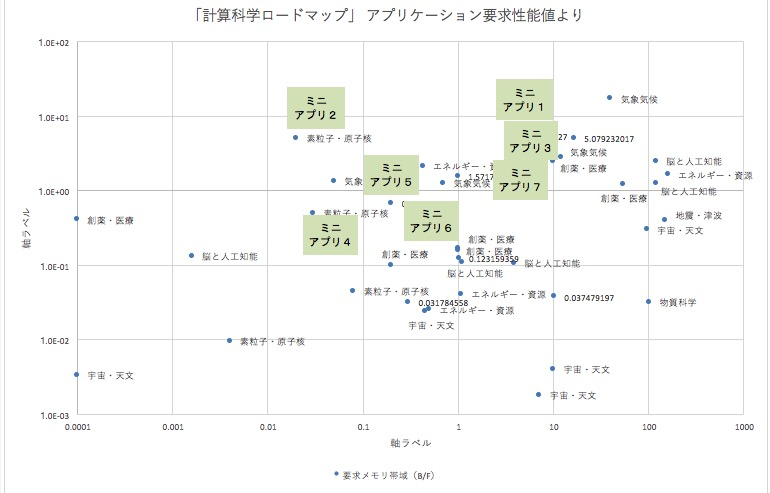
\includegraphics[clip]{figs/3-2-miniapps.jpg}
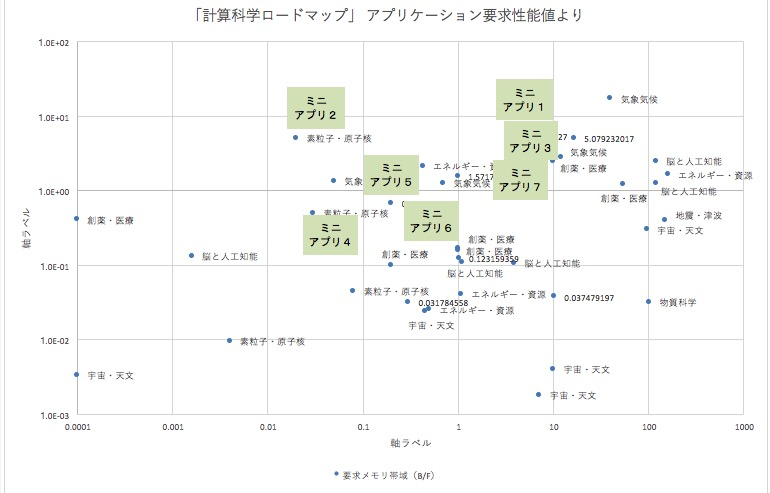
\includegraphics[width=\textwidth]{figs/3-2-miniapps.jpg}
\caption{2章アプリケーションとミニアプリの対応}
\label{fig:apps-miniapps}
\end{figure}


% 参考文献
\nocite{*}
\bibliographystyle{\rmbibstyle}
\bibliography{3-2}

